\section{Getting Started}

\noindent 
Each logic circuit, or sub-circuit, being designed with the Quartus Prime software is
called a {\it project}. Quartus Prime works on one project at a time
and keeps all information for that project in a single directory (folder) in
the file system.  To begin a new logic circuit design, the first step is
to create a directory to hold its files.  For this tutorial, we will use a directory 
named {\it introtutorial}. The running example for this tutorial is a simple circuit for 
two-way light control.

Start the Quartus Prime software. You should see a display
similar to the one in Figure~\ref{fig:2}. This display consists of several windows that 
provide access to all the features of the software, which the user selects with the 
computer mouse. Most commands in Quartus Prime can be accessed by using 
a set of menus that are located below the title bar. For example, in Figure~\ref{fig:2} 
clicking the left mouse button on the menu named {\sf File} opens the menu shown in 
Figure~\ref{fig:3}. Clicking the left mouse button on the entry {\sf Exit} exits
from Quartus Prime software. In general, whenever the mouse is used to select
something, the {\it left} button is used. Hence we will not normally
specify which button to press. In the few cases when it is
necessary to use the {\it right} mouse button, it will be specified explicitly. 

\begin{figure}[H]
   \begin{center}
      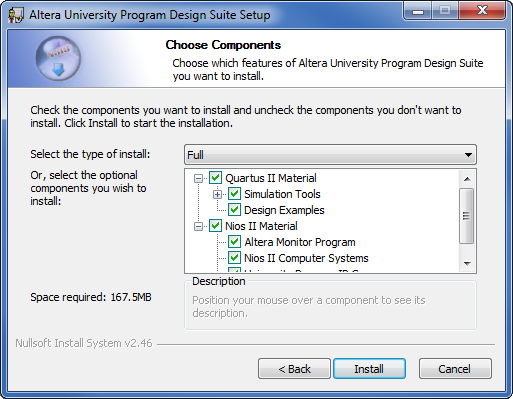
\includegraphics[scale=0.4]{figures/figure2.png}
   \caption{The main Quartus Prime display.} 
	 \label{fig:2}
	 \end{center}
\end{figure}

\begin{figure}[H]
   \begin{center}
      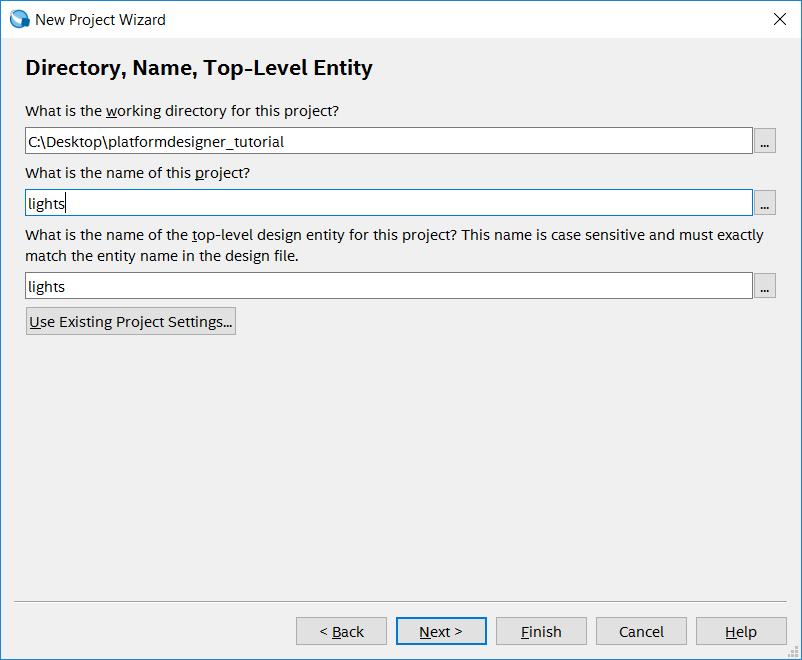
\includegraphics[scale=0.55]{figures/figure3.png}
   \caption{An example of the File menu.} 
	 \label{fig:3}
	 \end{center}
\end{figure}

\newpage
For some commands it is necessary to access two or more menus in sequence.
We use the convention {\sf Menu1 $>$ Menu2 $>$ Item} to indicate that 
to select the desired command 
the user should first click the left mouse button on {\sf Menu1}, then 
within this menu click on {\sf Menu2}, and then
within {\sf Menu2} click on {\sf Item}. For example, 
{\sf File $>$ Exit} uses the mouse to exit from the system.
Many commands can be invoked by clicking on an icon displayed in 
one of the toolbars. To see the command associated with an icon, position the mouse
over the icon and the command name will be shown in the status bar at the bottom of the screen.
